\section{Resultados}
\subsection{Información de los fármacos}

Tras la ejecución de nuestro flujo de bash con sus cuatro opciones, en la carpeta de resultados vamos a tener un directorio para cada combinación de fase del ensayo clínco y del conjunto de proteínas diana buscadas. En la carpeta encontramos dos archivos csv, uno contiene información genérica del fármaco (id de ChEMBL del fármaco y de la proteína objetivo, fecha de aprobación, etc.) y el otro corresponde a la información química de cada fármaco encontrado. 

En nuestro trabajo, no usamos la información química obtenida para analizar los fármacos resultates de nuestra búsqueda. Sin embargo, como vemos en \cite{Poleto2018} datos químicos como el número de anillos aromáticos pueden ser de gran ayuda a la hora de estudiar los efectos de un fármaco sobre el organismo. Por ello, guardamos esta información y definimos en el anexo el significado de cada variable de los archivos csv.


\subsection{Gráficas en R}
Tras obtener los datos de los fármacos para fase del ensayo clínico 3 y 4 y para proteínas del interactoma SARS-Humano y las proteínas secundarias, vamos a realizar una serie de gráficos que nos ayuden a analizarlos. A continuación, mostraremos solo aquellos correspondientes a los fármacos de fase cuatro debido a que los de fase tres nos porporcionan muy pocos resultados. 

Lo primero que creamos es una gráfica de barras en la que representamos la frecuencia de cada tipo de acción tanto para las proteínas de primer grado como para las de segundo. Con esto buscamos obtener unda idea de cuál es más viable para ser utilizado contra el COVID-19. Estos tipos de acción se refieren a la manera en la que el fármaco interactúa con la proteína o con su entorno.

\begin{figure}[h]
			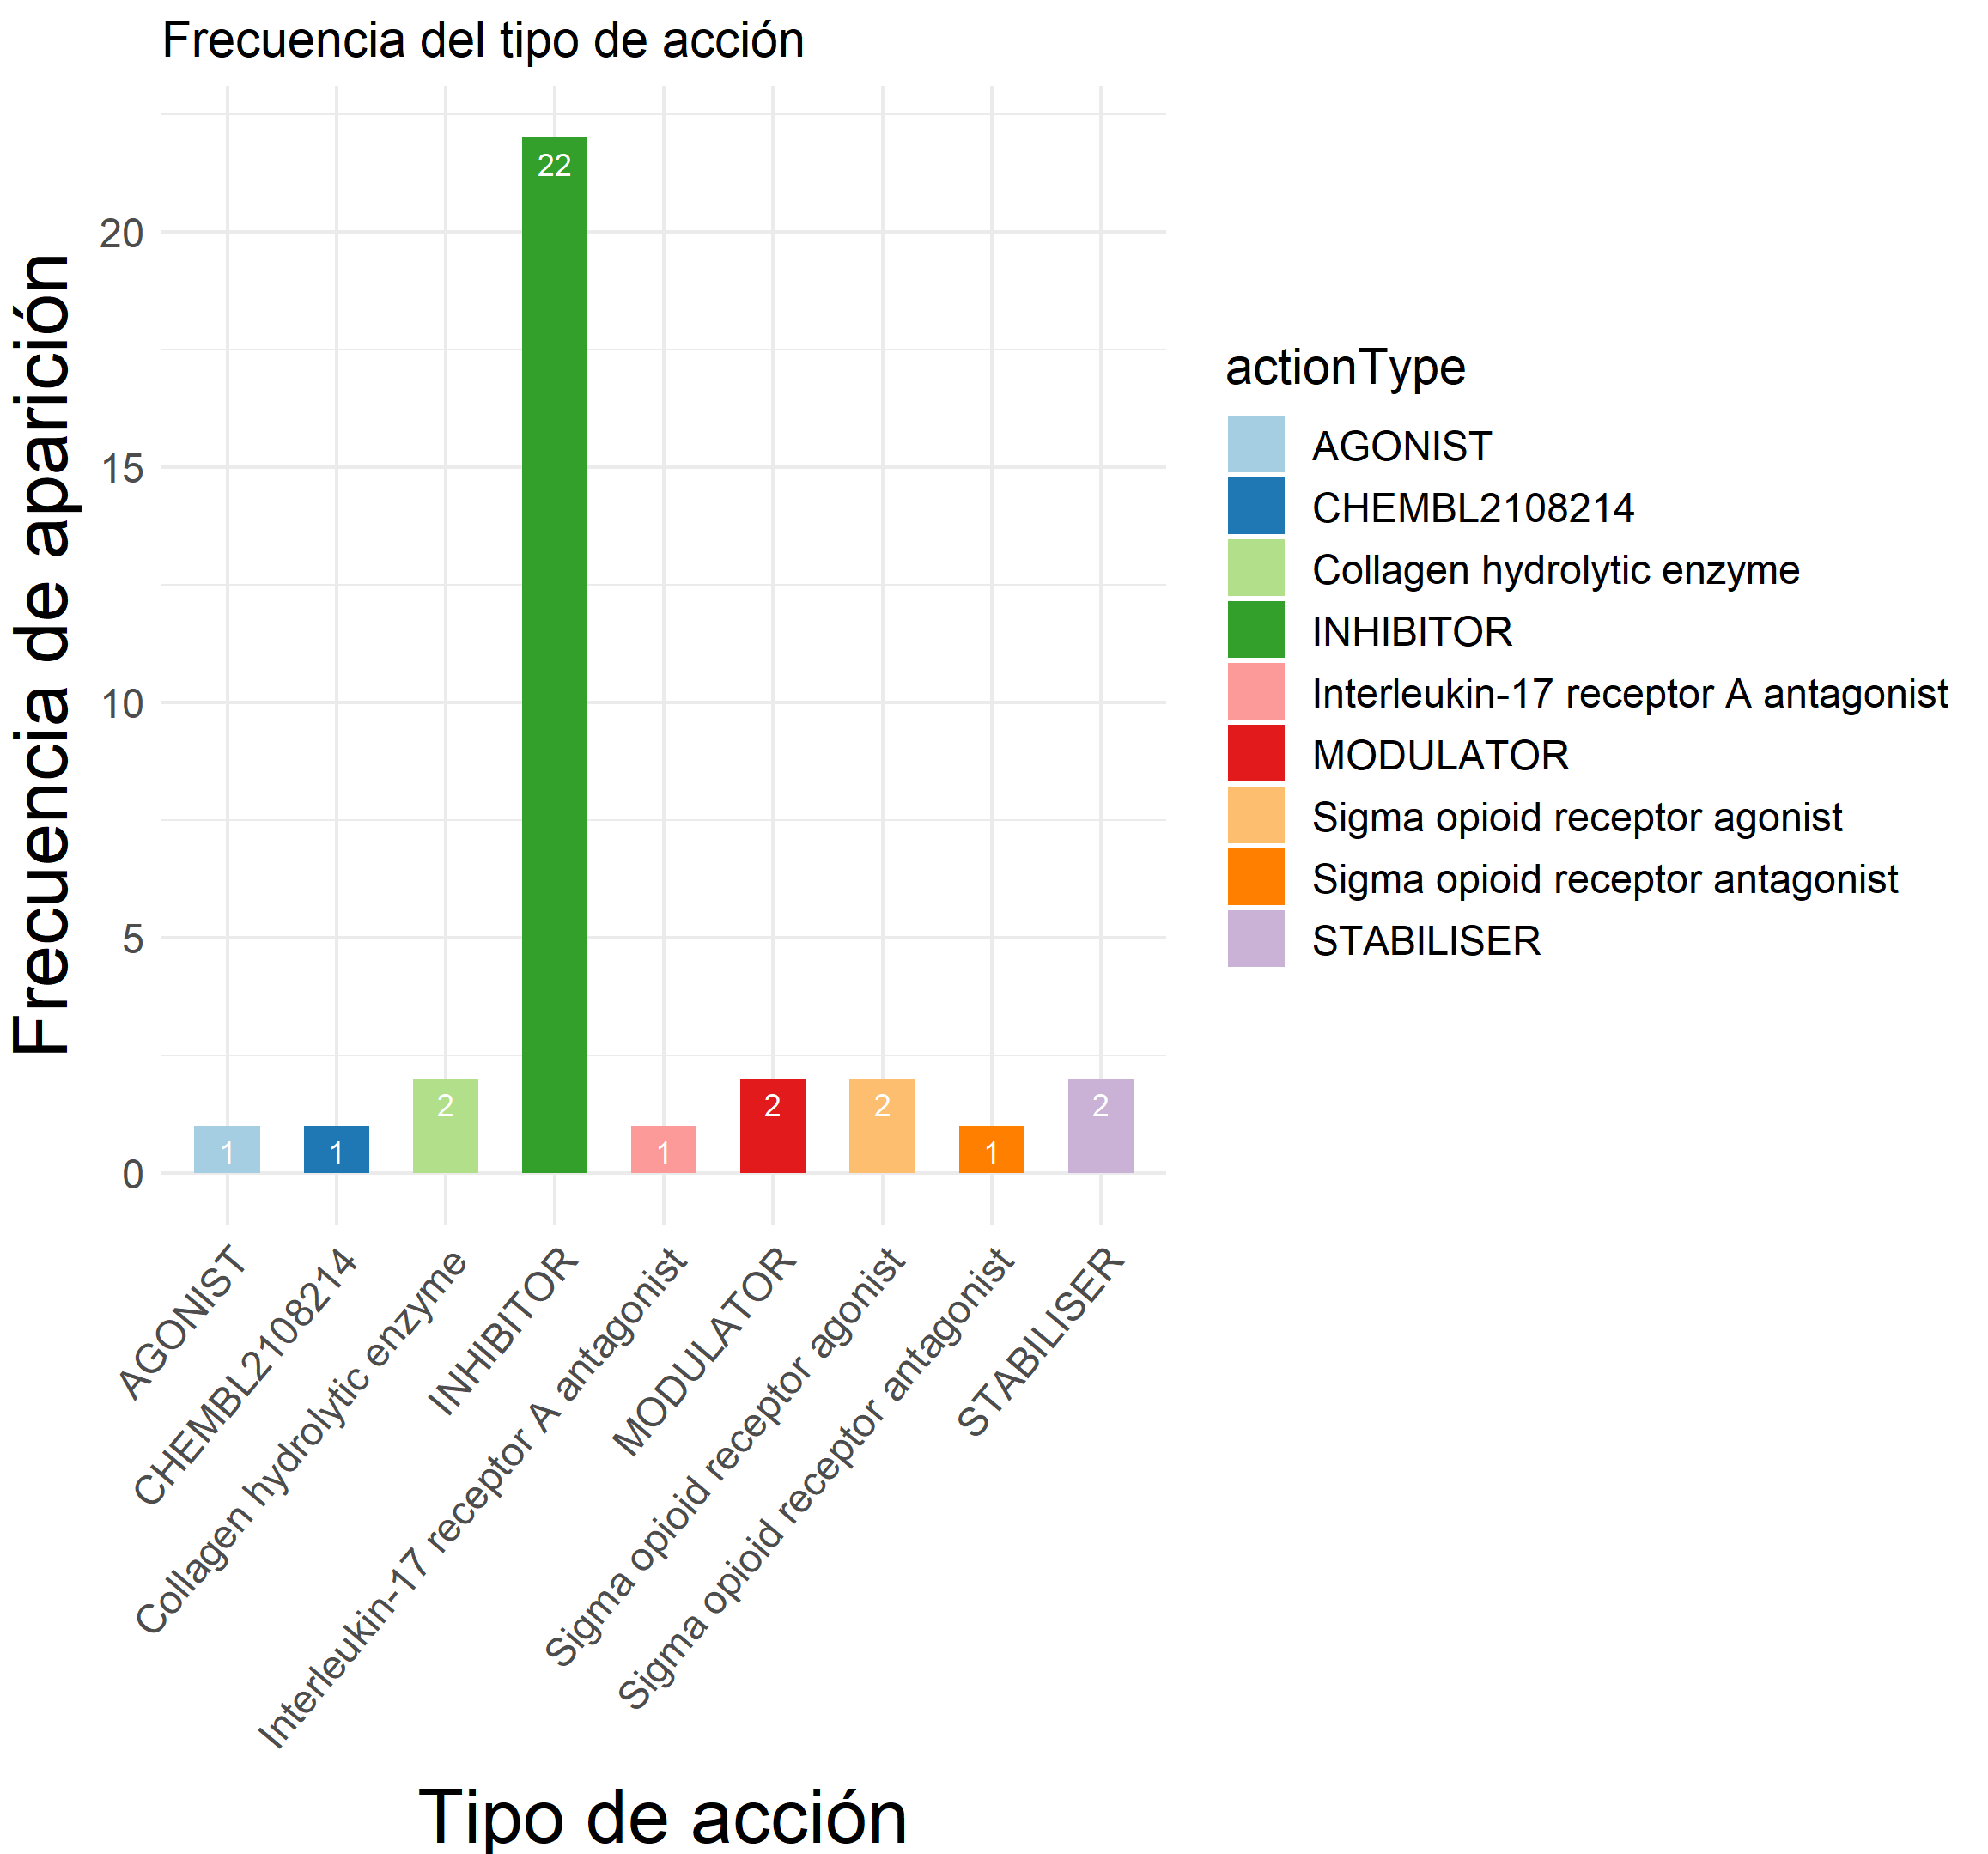
\includegraphics[width=0.9\textwidth]{figures/graficaTipoDeAccionProteinas1.png}
			\caption{Tipo de Acción, Proteínas de primer grado}
\end{figure}
\clearpage
\begin{figure}[h]
			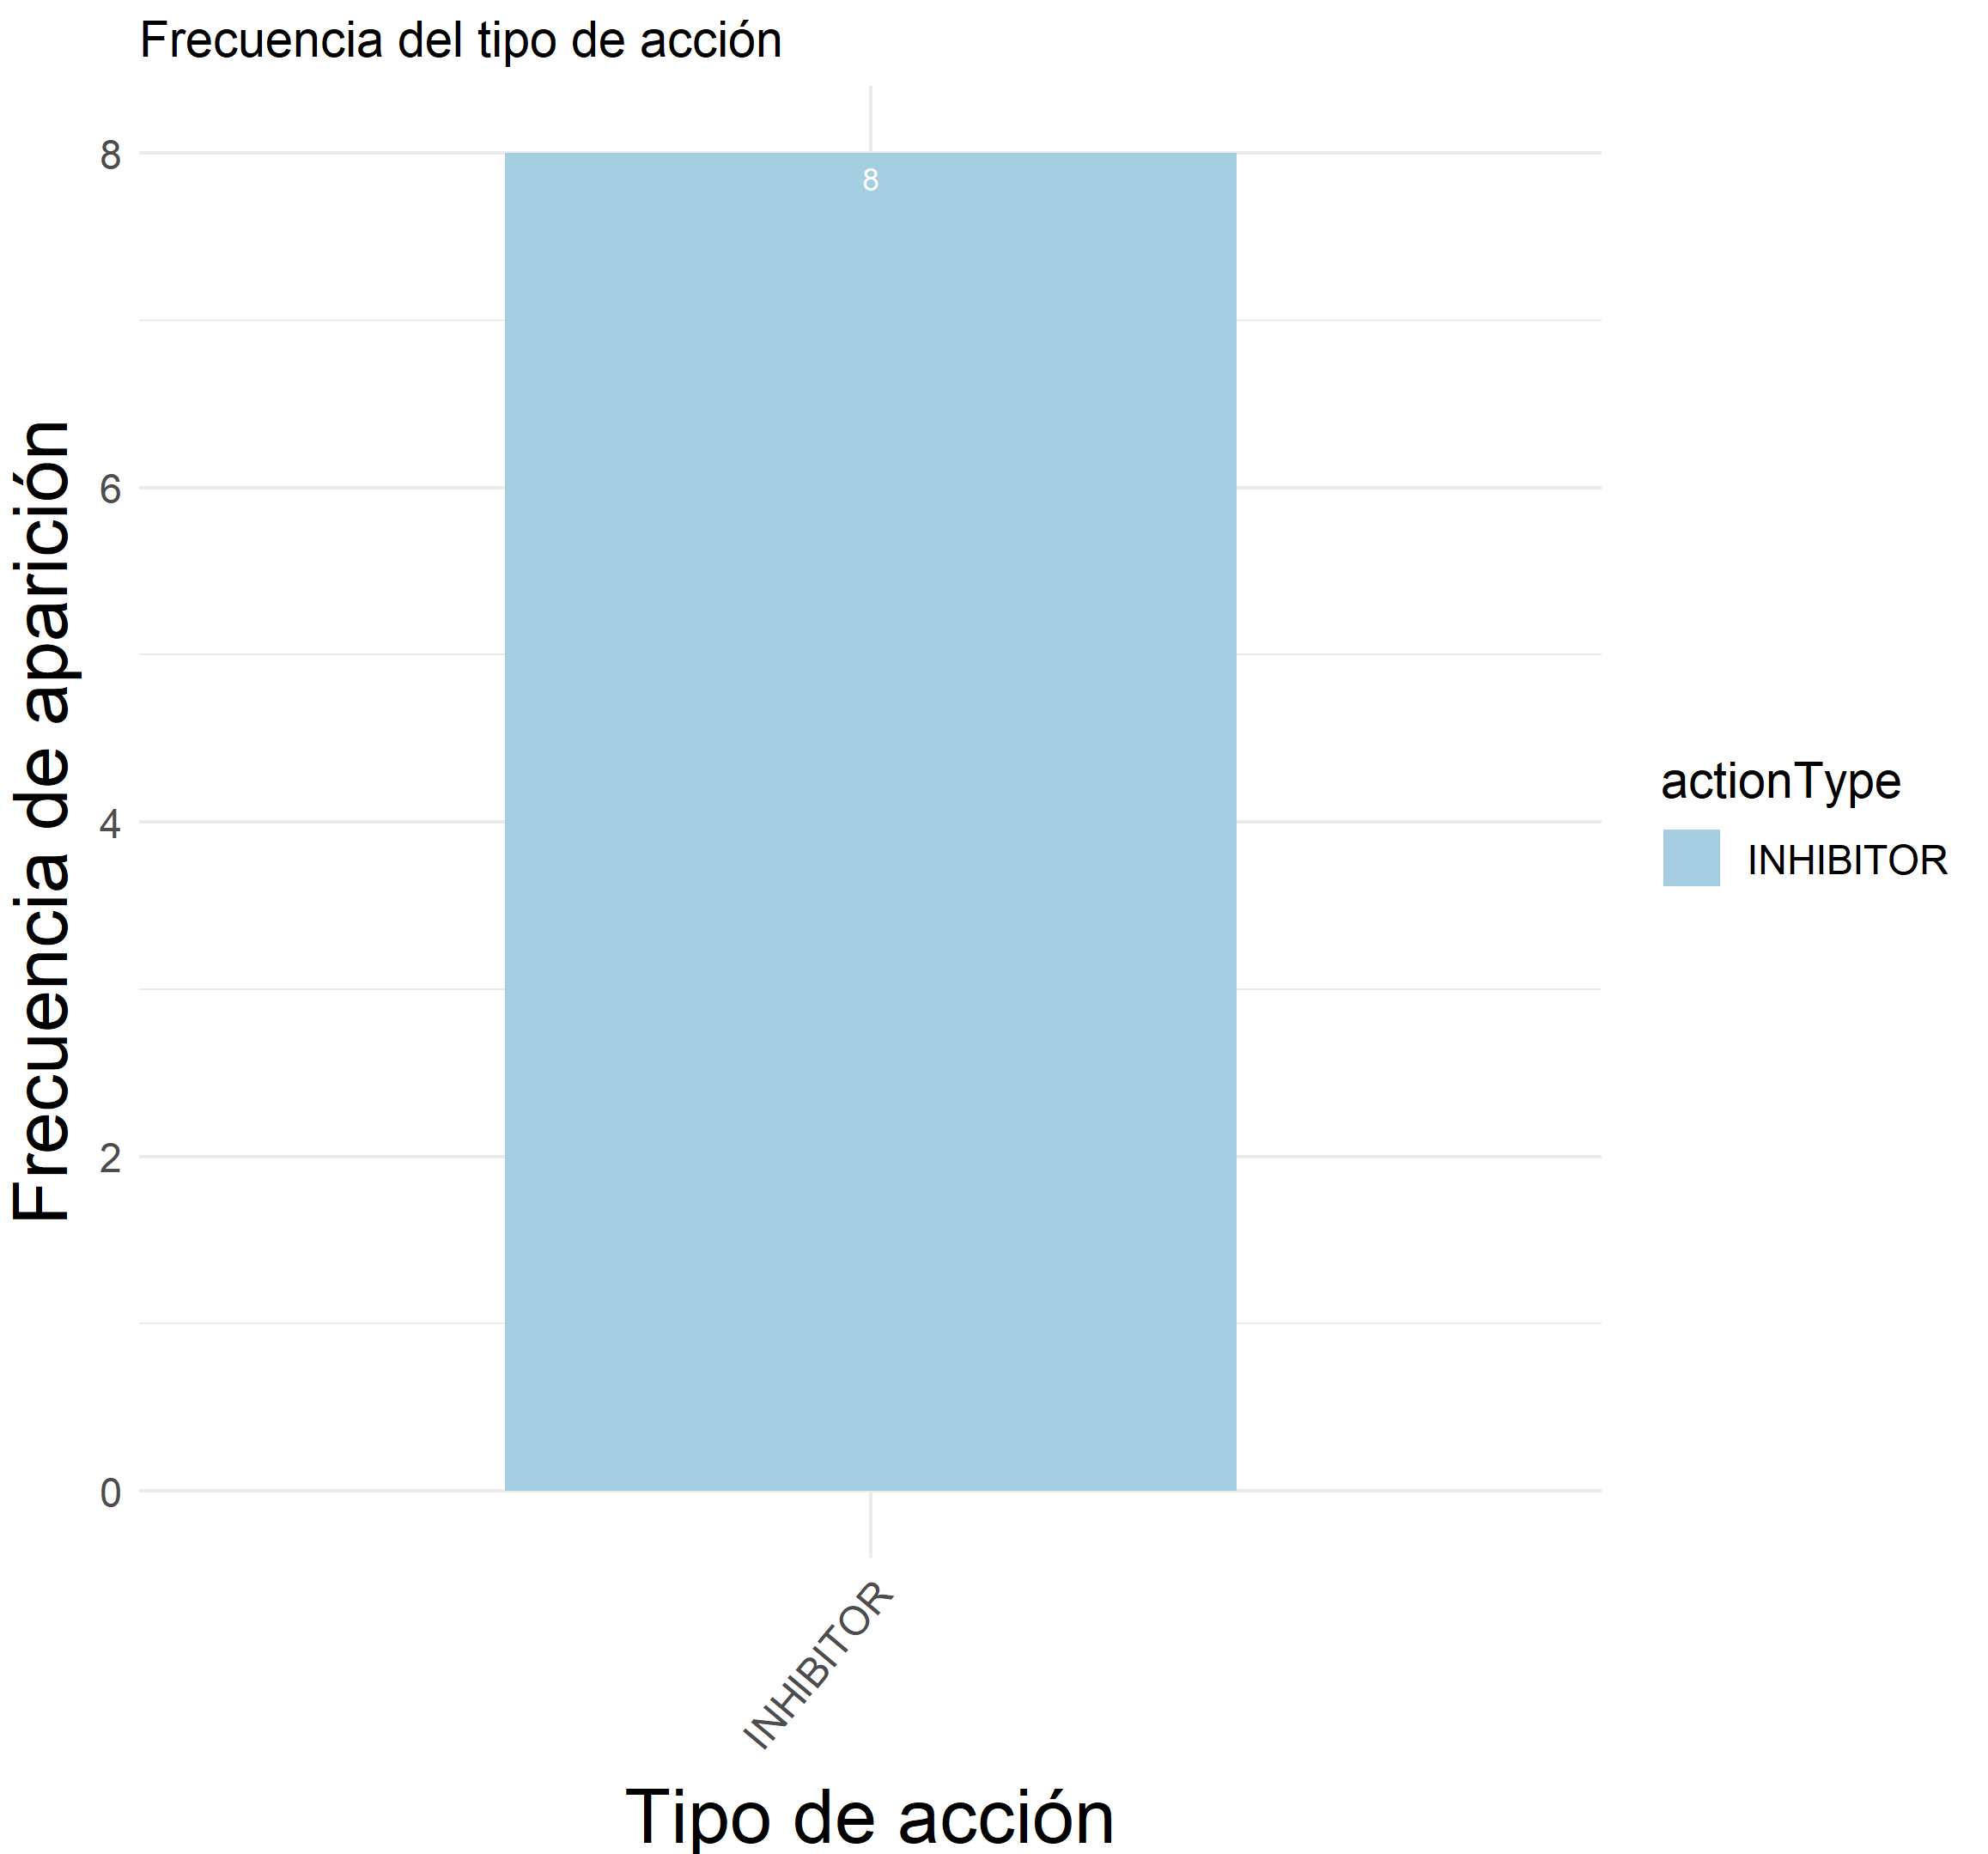
\includegraphics[width=0.9\textwidth]{figures/graficaTipoDeAccion.png}
			\caption{Tipo de Acción, Proteínas de segundo grado}
\end{figure}
%\clearpage 
%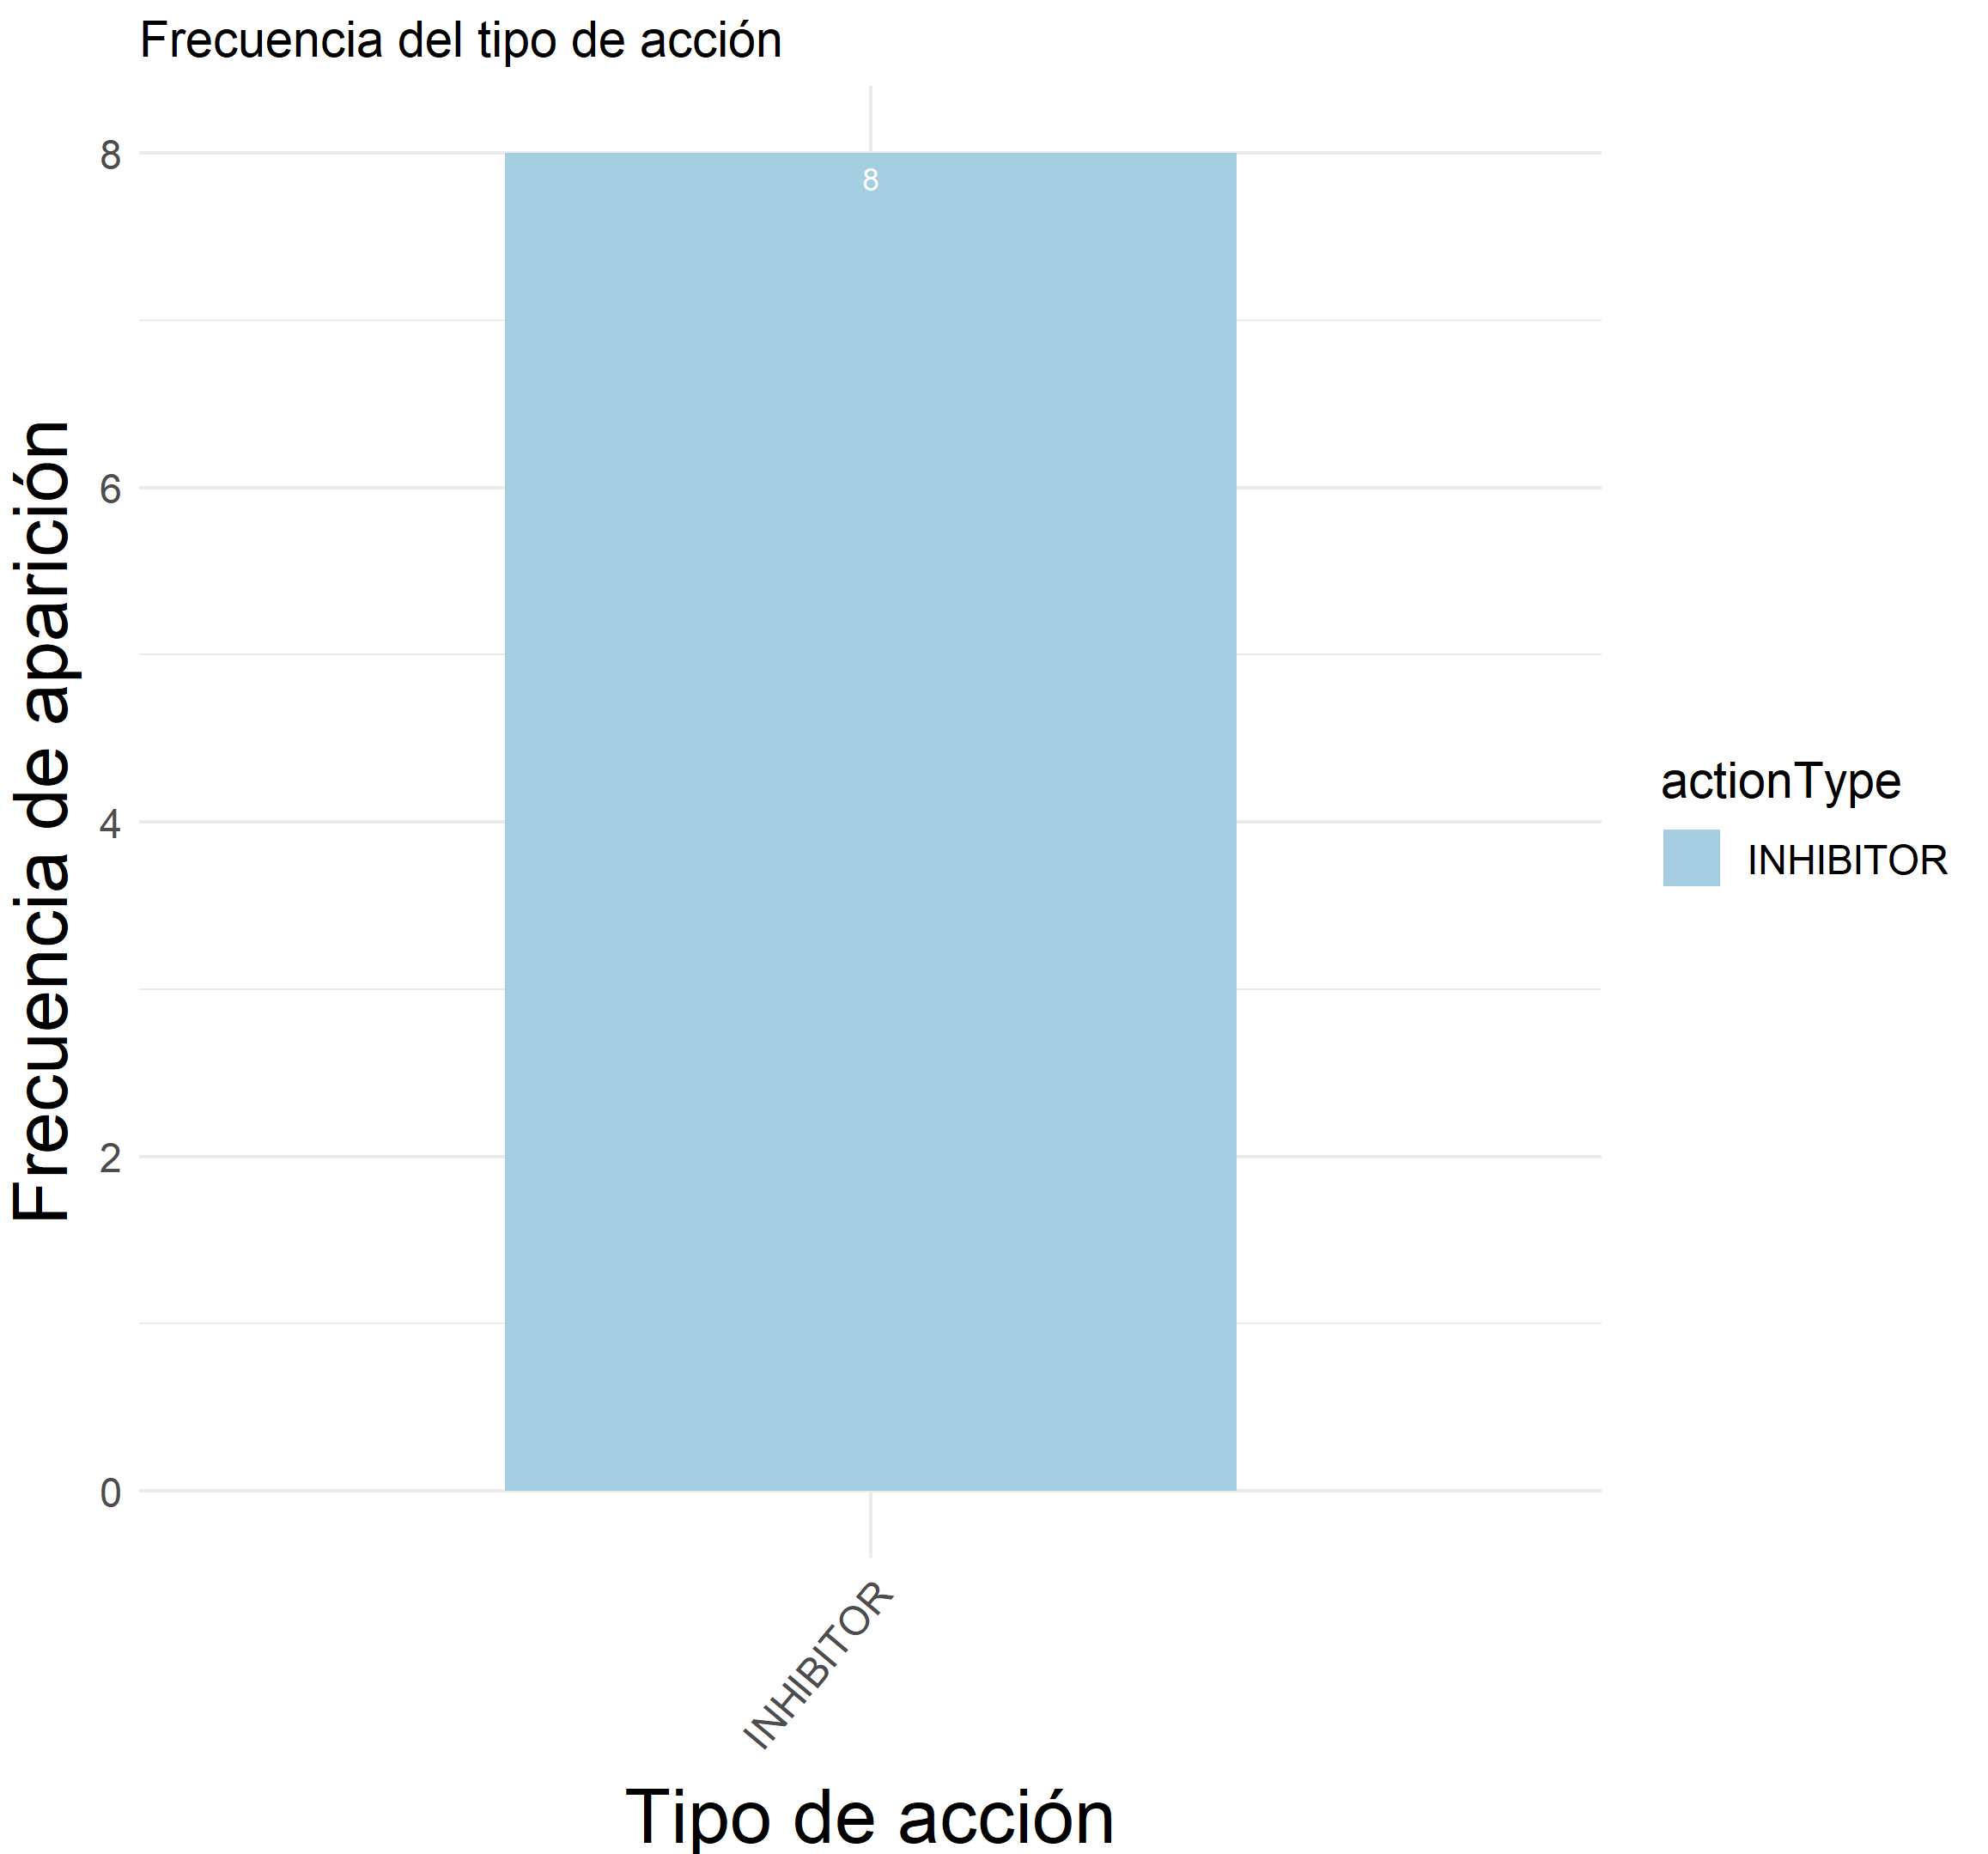
\includegraphics[width=\textwidth]{figures/graficaTipoDeAccion.png}\\
Como se puede comprobar, los inhibidores prevalecen. En el caso de las proteínas de primer grado, veintidós de los treinta y cuatro fármacos encontrados son inhibidores. En el caso de las de segundo grado, la totalidad de los fármacos (ocho) tiene acción inhibidora, significando esto que la mayoría de los fármacos encontrados para estas proteínas se dedican a reducir la actividad de enzimas de manera reversible, acoplándose a ellas.
	
Las siguientes dos gráficas muestran la frecuencia de cada mecanismo de acción existente. Conocer el mecanismo de acción de un fármaco aumenta la información conocida sobre su tipo de acción, pues especifica con mayor profundidad la actividad del fármaco sobre la proteína y la reacción del paciente a él. Con esto podremos ver si algún mecanismo de acción es muy común.

%\clearpage 

\begin{figure}[h!]
			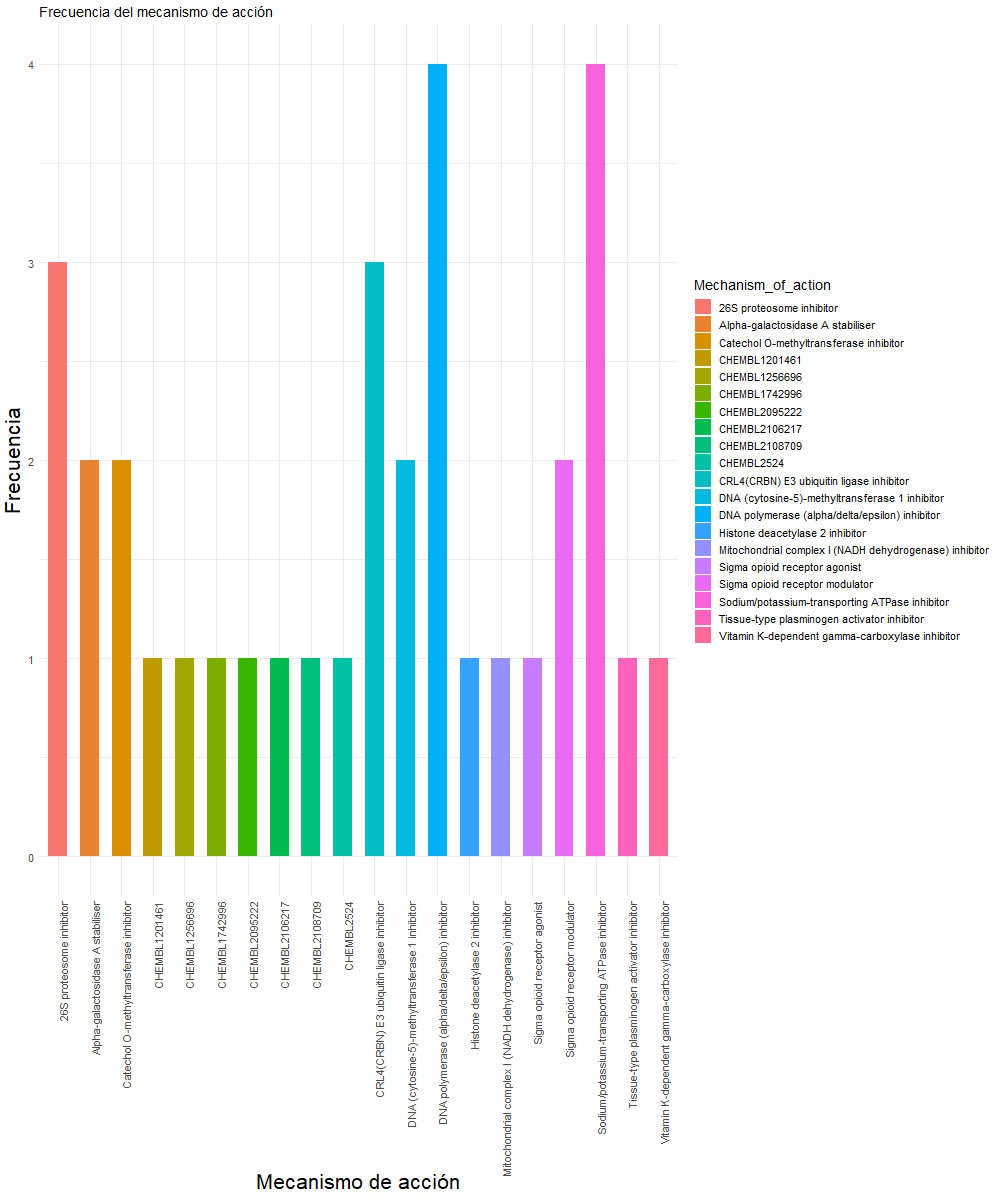
\includegraphics[width=0.9\textwidth]{figures/graficaMecanismoDeAccionProteinas1.png}
			\caption{Mecanismo de Acción, Proteínas de primer grado}
\end{figure}
\clearpage
\begin{figure}[h!]
			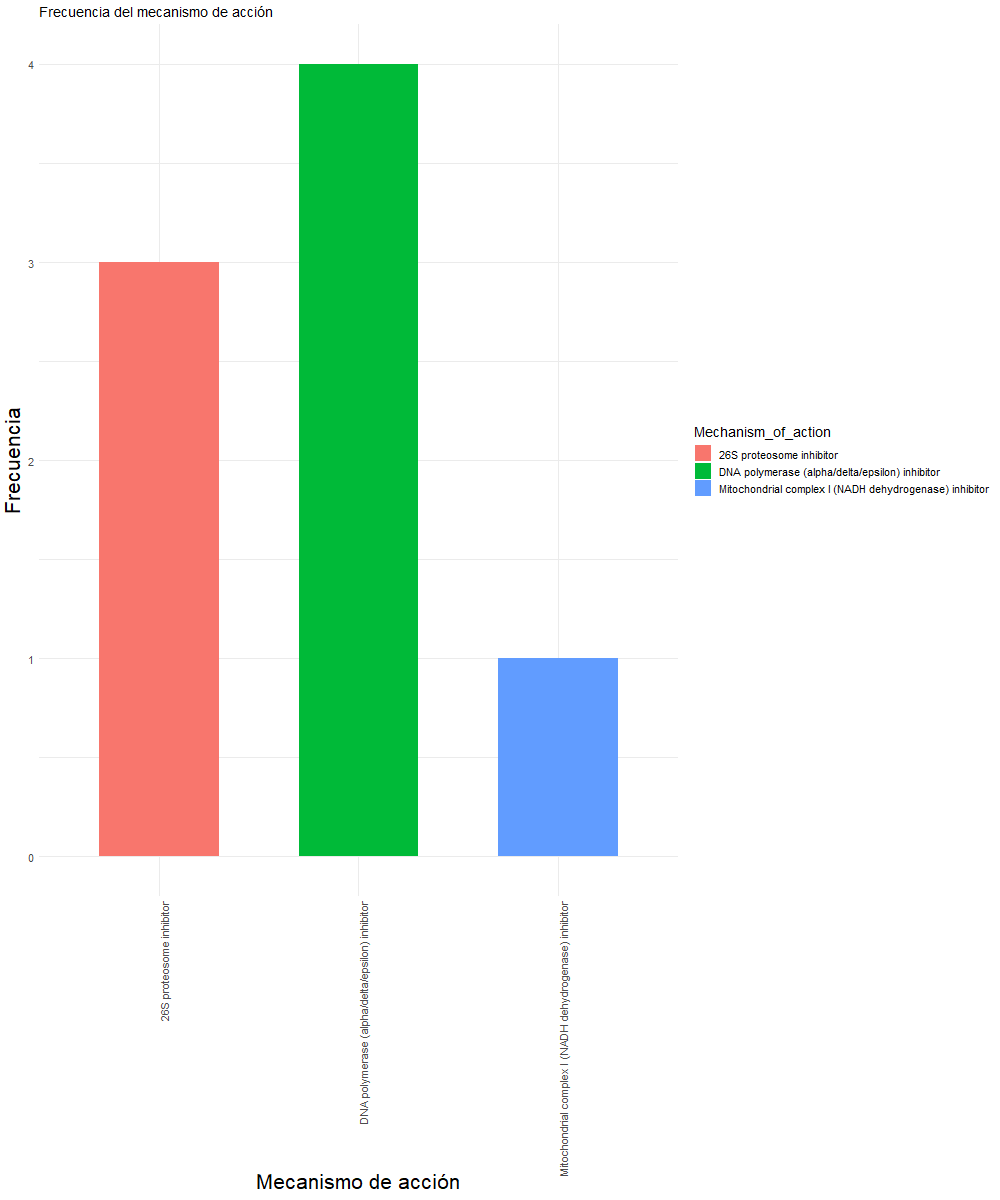
\includegraphics[width=0.9\textwidth]{figures/graficaMecanismoDeAccion.png}
			\caption{Mecanismo de Acción, Proteínas de segundo grado}
\end{figure}

%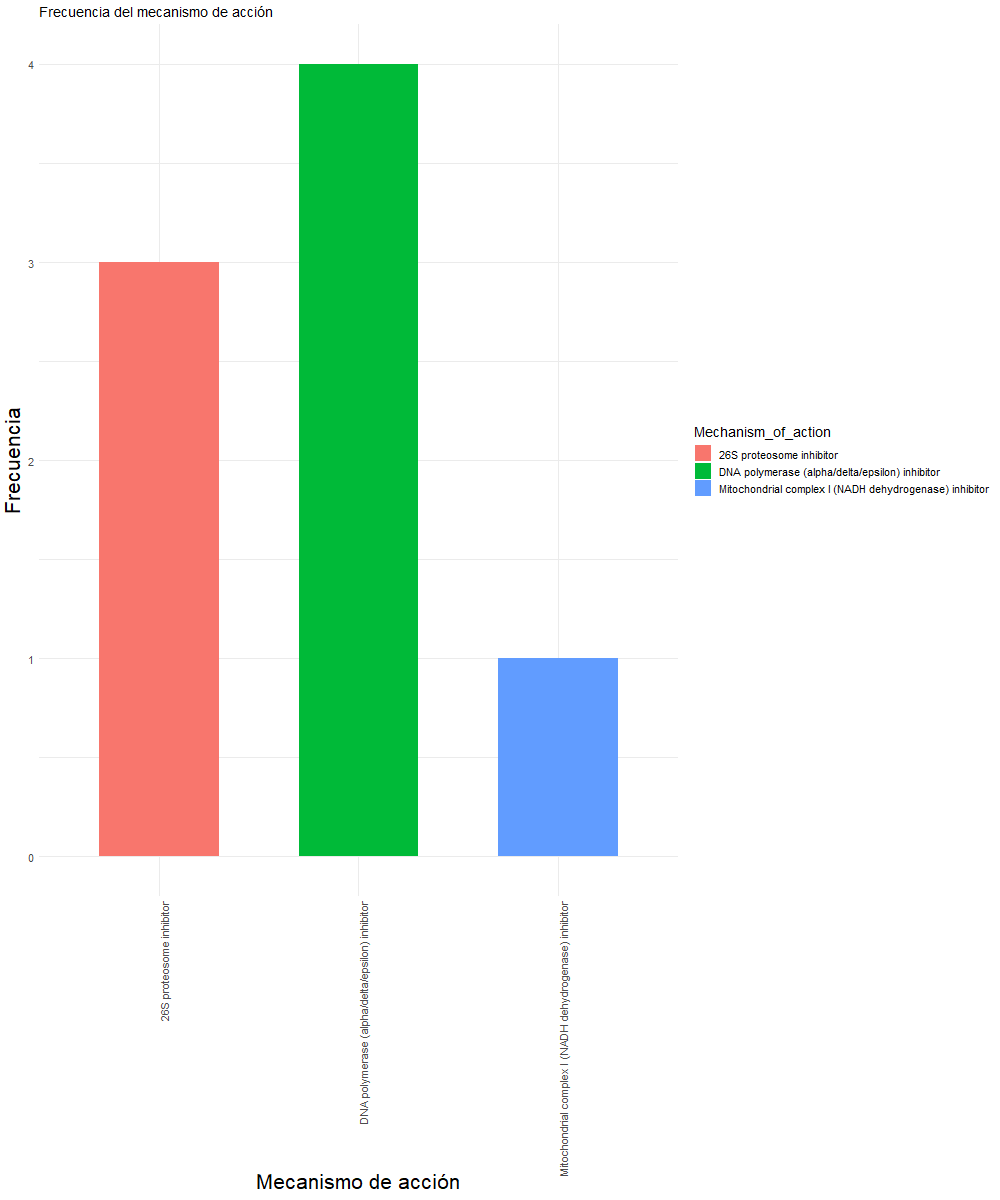
\includegraphics[width=\textwidth]{figures/graficaMecanismoDeAccion.png}\\

%\clearpage 
%\newpage

Observando estas gráficas podemos ver que para las proteínas de primer grado existen cuatro grupos principales de inhibidores, que actúan sobre el proteasoma 26S, la ubiquitina ligasa, la DNA polimerasa y la ATPasa transportadora de sodio y potasio. Otros mecanismos de los que encontramos repeticiones son los estabilizadores de alfa-galactosidasa, inhibidores de metiltransferasa y moduladores de receptor opioide.

En el caso de las proteínas de segundo grado, volvemos a encontrarnos con cuatro fármacos que inhiben a la DNA polimerasa, y tres al proteasoma 26S, además de una que inhibe al complejo mitocondrial. Que se repitan dos mecanismos en ambos tipos de proteínas podría indicar la relevancia de ellos.

Por último, representaremos redes que reflejan la relación entre proteínas y los medicamentos que las afectan. Por tanto podremos encontrar proteínas con mayor cantidad de medicamentos que las puedan afectar.

\begin{figure}[h]
			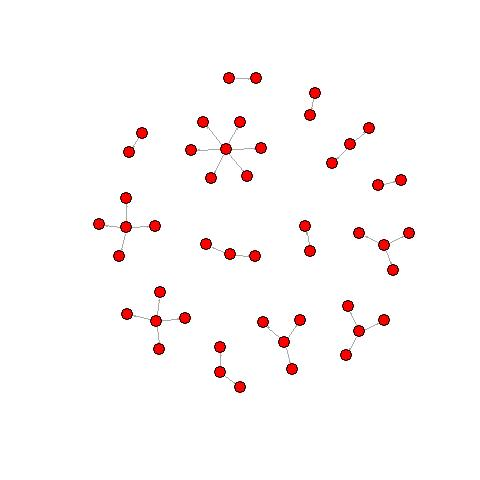
\includegraphics[width=0.9\textwidth]{figures/Red-medicamento-proteina1.jpeg}
			\caption{Interacción proteína-medicamento, Proteínas de primer grado}
\end{figure}
\clearpage
\begin{figure}[h]
			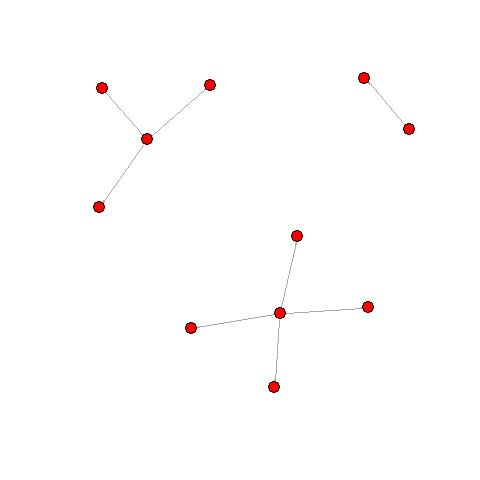
\includegraphics[width=0.9\textwidth]{figures/Red-medicamento-proteina2.jpeg}
			\caption{Interacción proteína-medicamento, Proteínas de segundo grado}
\end{figure}

%\clearpage
A partir de estas redes podemos ver que del primer grupo de proteínas extraemos catorce proteínas relacionadas con nuestros treinta y cuatro fármacos, de las que destaca una con seis medicamentos que la tienen como objetivo.

En el segundo grupo solo se localizan fármacos para tres de las proteínas, pues a dos de ellas las afecta más de un fármaco.

\newpage
		